\section{Охрана Труда. Безопасность инженеров разработчиков на предприятии малого бизнеса Акавита}

Целью дипломного проекта явилась разработка алгоритмов, которые способствуют улучшению выдачи поисковых систем, путём обучения и анализа поведения пользователей. Техническая суть состоит в создании и разработке алгоритмов которые смогут быть применены на разных типах данных для улучшения релевантности выдачи поисковых систем. Разработка выполнена на предприятии “Акавита”.

В настоящем разделе рассмотрены вопросы, связанные с обеспечением безопасных условий труда инженеров-разработчиков на предприятии малого бизнеса “Акавита”.

Заместителем начальника по управлению кадрами были проведены организационные и инженерно-технические мероприятия по пожарной безопасности. Кроме этого, определен порядок обесточивания электрооборудования по окончании рабочего дня и в случае пожара. Начальник отдела разработки обеспечил пожарную безопасность и противопожарный режим в компании, посредством правильной организации рабочих мест и плана эвакуации. План эвакуации помещения инженеров- 	разработчиков приведен на рисунке ~\ref{evacuation_plan}.

Важную роль в обеспечении пожарной безопасности играет персонал. В компании “Акавита” обучение персонала проводится путем его инструктирования и прохождения пожарно-технического минимума. В связи с законодательством Республики Беларусь ~\cite{ot_1} и приказом директора компании был определен порядок и сроки противопожарного инструктажа и пожарно-технического минимума, а также назначены лица, ответственные за
их проведение. 

\begin{figure}
  \centering
  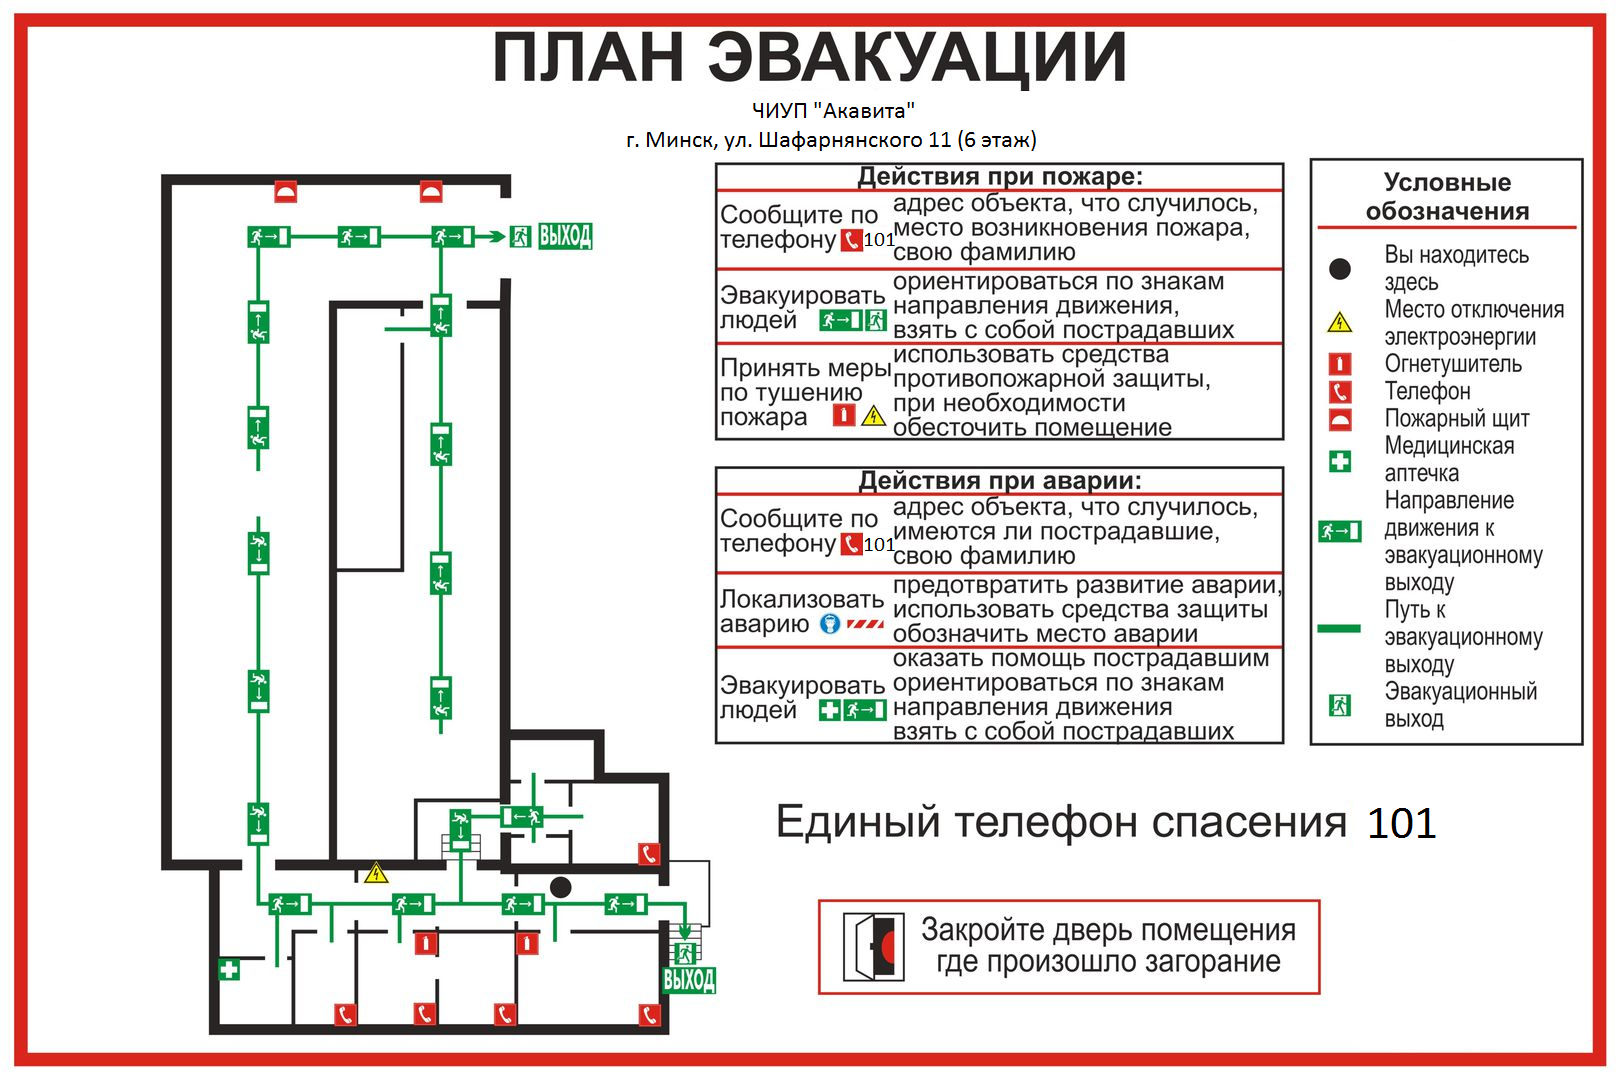
\includegraphics[width=0.9\textwidth]{images/evacuation_plan.png}
  \caption{План Эвакуации разработчиков отдела инженеров-разработчиков в ЧИУП Акавита\label{evacuation_plan}}
\end{figure}

На первичном инструктаже было рассказано об оборудовании, используемом на предприятии, в частности был проведен инструктаж о том, как пользоваться персональным компьютером, принтером, и другим электрическим оборудованием. Были указаны места для курения. Также, были показаны места расположения телефонов и объяснены правила поведения в случае возникновения пожара. 

На предприятии “Акавита” имеются следующие территории: коридор, переговорный зал, игровая комната, отдел разработчиков, отдел тестировщиков, отдел бизнес аналитиков. Для каждого помещения были назначены люди, ответственные за пожарную безопасность этих помещений, а также технологического и инженерного оборудования.

На каждый огнетушитель, установленный на предприятии “Акавита” заведен паспорт. У огнетушителя есть порядковый номер, который нанесен краской на огнетушитель, он записан в эксплуатационный паспорт огнетушителя и в журналы по техническому обслуживанию огнетушителей. Огнетушители размещаются на расстоянии 1.4 м от проёма двери и на высоте 0.2 м.

Чтобы обеспечивалось удобство зрительного наблюдения, быстрое и точное считывание информации, плоскость экрана монитора располагается ниже уровня глаз инженера-разработчика практически перпендикулярно к нормальной линии взгляда работника. Для исключения воздействия повышенных уровней электромагнитных излучений расстояние между экраном монитора и работником составляет не менее 500 мм ~\cite{ot_2}. Рабочий стул (кресло) имеет устойчивое положение, место сидения регулируется по высоте, а спинка сиденья - по высоте, углам наклона, а также расстоянию спинки от переднего края сиденья. Регулировка каждого параметра независима, легко осуществляема и имеет надежную фиксацию. Клавиатура располагается на поверхности стола таким образом, чтобы пространство перед клавиатурой было достаточным для опоры рук инженера-разработчика (на расстоянии не менее чем 350 мм от края, обращенного к работнику ~\cite{ot_2}).

\begin{figure}
  \centering
  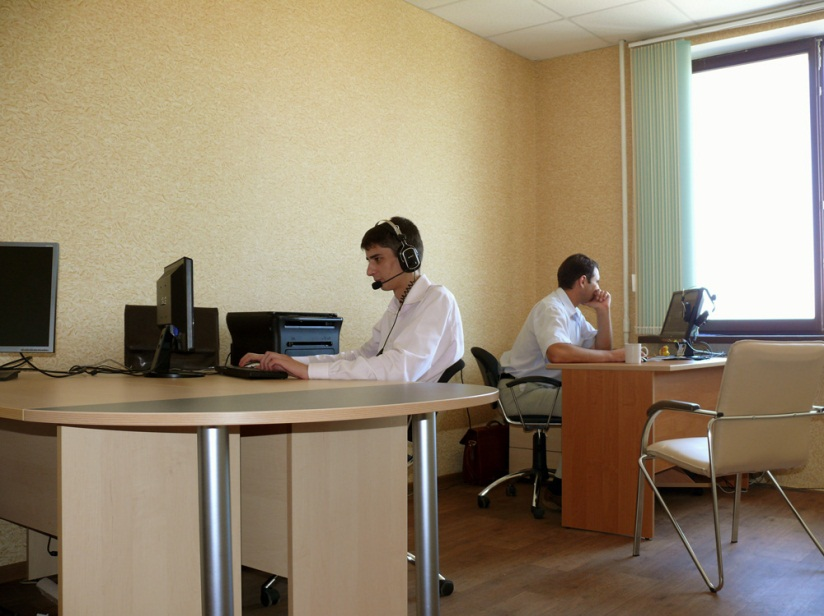
\includegraphics[width=0.9\textwidth]{images/work_place.jpg}
  \caption{рабочее место инженера-разработчика в ЧИУП «Акавита»\label{work_place}}
\end{figure}

Рабочее место размещается таким образом, чтобы естественный свет падал сбоку. Для снижения яркости в поле зрения при естественном освещении применяются регулируемые жалюзи, плотные шторы. Возможные мешающие отражения и отблески на экране монитора и другом оборудовании устраняются путем соответствующего размещения экрана, оборудования, расположения светильников местного освещения. Для обеспечения безопасности инженеров-разработчиков на соседних рабочих местах расстояние между рабочими столами с мониторами составляет 1,5 м, а расстояние между боковыми поверхностями мониторов - 1,4 м ~\cite{ot_2}. Для обеспечения оптимальных параметров микроклимата проводится регулярное в течение рабочего дня проветривание и ежедневная влажная уборка помещений, используются увлажнители воздуха.

При работе с персональным компьютером инженеры-разработчики должны соблюдать режим труда и отдыха, установленный законодательством, правилами внутреннего трудового распорядка организации, трудовую дисциплину, выполнять требования охраны труда, правил личной гигиены. Кроме того, программисты должны выполнять требования пожарной безопасности, знать порядок действий при пожаре, уметь применять первичные средства пожаротушения. Курение производится только в специально предназначенных для курения местах. Особенно важно сообщать о неисправностях оборудования и других замечаниях по работе с персональным компьютером непосредственному руководителю или лицам, осуществляющим техническое обслуживание оборудования. Пример рабочего места в компании «Акавита» приведен на рисунке ~\ref{work_place}.


Таким образом, изложенные выше предложения обеспечат безопасность труда инженеров-разработчиков на предприятии малого бизнеса «Акавита».

